\documentclass[../DoAn.tex]{subfiles}
\begin{document}

Chương này trình bày quá trình khảo sát hiện trạng và xác định yêu cầu cho hệ thống multi-tenant RAG chatbot hỗ trợ tư vấn bán hàng nội thất. Nội dung chương bắt đầu từ việc phân tích nhu cầu của người dùng cuối, cửa hàng nội thất và quản trị hệ thống, đồng thời xem xét một số nhóm giải pháp hiện có như chatbot kịch bản, chatbot chăm sóc khách hàng, AI agent thương mại và các hệ thống bán hàng trực tuyến có chức năng tìm kiếm, lọc sản phẩm. Từ kết quả khảo sát, chương xác định các hạn chế cần khắc phục và khái quát các chức năng chính của hệ thống.

Tiếp theo, chương trình bày tổng quan chức năng thông qua các tác nhân và use case chính, bao gồm tư vấn sản phẩm theo cửa hàng, quản lý chatbot và knowledge base, quản lý hội thoại, lead, yêu cầu mua hàng, tham chiếu giá cơ bản, tích hợp kênh chat ngoài và quản lý vận hành hệ thống. Các use case quan trọng được đặc tả ở mức chi tiết hơn để làm rõ luồng xử lý, tiền điều kiện và hậu điều kiện. Cuối cùng, chương đưa ra các yêu cầu phi chức năng liên quan đến hiệu năng, độ tin cậy, tính dễ sử dụng, khả năng bảo trì, bảo mật và khả năng mở rộng của hệ thống.

\section{Khảo sát hiện trạng}
\label{section:2.1}

Đối tượng sử dụng chính của hệ thống trong đồ án gồm người mua hàng nội thất, cửa hàng nội thất nhỏ và vừa, nhân viên cửa hàng, quản trị cửa hàng và quản trị hệ thống. Với người mua hàng, nhu cầu thường gặp không chỉ là tìm một sản phẩm theo tên hoặc mức giá, mà còn là được tư vấn theo bối cảnh sử dụng cụ thể. Ví dụ, người dùng có thể cần một bàn làm việc cho phòng nhỏ, một ghế sofa phù hợp với phòng khách hiện đại, hoặc một tủ có kích thước phù hợp với diện tích đang có. Trong quá trình trao đổi, người dùng có thể thay đổi ngân sách, thay đổi loại sản phẩm, yêu cầu gợi ý lại, từ chối đề xuất trước đó hoặc muốn tham khảo thêm thông tin về mức giá trước khi quyết định. Vì vậy, nhu cầu thực tế của người dùng là một quá trình tư vấn nhiều lượt, có ngữ cảnh, thay vì một lượt hỏi đáp đơn giản.

Đối với cửa hàng nội thất nhỏ và vừa, nhu cầu chính là có một công cụ hỗ trợ tư vấn khách hàng dựa trên dữ liệu sản phẩm hoặc tài liệu riêng của cửa hàng. Dữ liệu sản phẩm nội thất thường bao gồm nhiều thuộc tính như tên sản phẩm, mô tả, giá, chất liệu, kích thước, loại sản phẩm, phong cách, tên cửa hàng và liên kết sản phẩm. Khi số lượng sản phẩm tăng hoặc thông tin sản phẩm thay đổi, việc tư vấn thủ công có thể thiếu nhất quán, phụ thuộc vào kinh nghiệm của từng nhân viên và khó duy trì phản hồi nhanh trên nhiều kênh. Ngoài ra, không phải cửa hàng nào cũng có đội ngũ kỹ thuật để tự xây dựng, cập nhật và vận hành một hệ thống chatbot AI độc lập. Do đó, một nhu cầu quan trọng là cửa hàng có thể quản lý chatbot, nguồn dữ liệu knowledge base, hội thoại, lead và yêu cầu mua hàng thông qua giao diện quản trị.

Hiện nay, một nhóm công cụ phổ biến cho bán hàng trực tuyến là chatbot kịch bản và chatbot marketing. Nhóm công cụ này phù hợp với các tình huống tương tác có luồng xử lý rõ ràng như chào hỏi, thu thập thông tin liên hệ, gửi thông báo hoặc trả lời một số câu hỏi thường gặp. Ưu điểm của nhóm giải pháp này là dễ tiếp cận, triển khai nhanh và dễ kiểm soát nội dung trong các kịch bản đơn giản. Tuy nhiên, khi áp dụng vào bài toán tư vấn nội thất, hạn chế chính là tính phụ thuộc vào luồng hội thoại được thiết kế trước. Nếu khách hàng thay đổi yêu cầu, đặt câu hỏi theo cách không dự đoán trước, hoặc cần tiếp tục trao đổi theo ngữ cảnh trước đó, chatbot kịch bản khó duy trì được một quá trình tư vấn linh hoạt.

Một nhóm công cụ khác là các nền tảng live chat và chatbot hỗ trợ chăm sóc khách hàng. Các hệ thống này có ưu điểm ở khả năng kết hợp giữa chatbot và nhân viên thật, giúp doanh nghiệp phản hồi khách hàng nhanh hơn và xử lý các câu hỏi phổ biến hiệu quả hơn. Tuy nhiên, với bài toán của đồ án, nhu cầu không chỉ là trả lời nhanh mà còn là tư vấn theo dữ liệu riêng của từng cửa hàng, duy trì ngữ cảnh hội thoại, ghi nhận nhu cầu mua hàng và chuyển các thông tin phát sinh thành lead hoặc yêu cầu mua hàng để cửa hàng tiếp tục xử lý. Các nền tảng live chat tổng quát thường tập trung vào hỗ trợ khách hàng nói chung, trong khi đề tài tập trung vào một quy trình tư vấn bán hàng nội thất trong môi trường nhiều cửa hàng.

Các nền tảng xây dựng AI agent hoặc chatbot có knowledge base phù hợp hơn với những bài toán cần truy xuất thông tin từ dữ liệu có sẵn. Nhóm giải pháp này có khả năng xây dựng chatbot dựa trên nguồn tri thức riêng, hỗ trợ tích hợp với nhiều hệ thống và phù hợp hơn với các bài toán hỏi đáp theo dữ liệu. Tuy nhiên, việc xây dựng knowledge base, cấu hình luồng xử lý, kiểm soát chất lượng truy xuất và duy trì dữ liệu thường vẫn cần hiểu biết kỹ thuật nhất định. Với các cửa hàng nội thất nhỏ và vừa, đây là một rào cản đáng kể, đặc biệt khi họ cần một hệ thống có thể sử dụng trên dữ liệu riêng mà không phải tự thiết kế toàn bộ pipeline AI.

Bên cạnh đó, các AI agent thương mại phục vụ chăm sóc khách hàng, bán hàng và thương mại điện tử hiện nay đã có mức độ hoàn thiện cao. Các nền tảng thuộc nhóm này có thể hỗ trợ trả lời dựa trên knowledge base, tích hợp nhiều kênh, chuyển tiếp cho nhân viên và tự động hóa một số tác vụ trong quy trình chăm sóc khách hàng. Vì vậy, các hệ thống này không nên được xem là chatbot hỏi đáp đơn giản, mà là các nền tảng AI agent tổng quát. Trong phạm vi đồ án, hệ thống không đặt mục tiêu cạnh tranh trực tiếp với các nền tảng thương mại như vậy về quy mô, số lượng kênh tích hợp hoặc mức độ tự động hóa nghiệp vụ. Trọng tâm của đồ án là xây dựng một hệ thống có phạm vi hẹp hơn, tập trung vào tư vấn bán hàng nội thất trong môi trường nhiều cửa hàng, quản lý chatbot và knowledge base theo từng tenant, ghi nhận lead/yêu cầu mua hàng từ hội thoại và hỗ trợ tham chiếu giá cơ bản trong phạm vi dữ liệu của hệ thống.

Ngoài các nền tảng chatbot, các website thương mại điện tử và website bán hàng nội thất thường cung cấp chức năng tìm kiếm, lọc và sắp xếp sản phẩm theo một số tiêu chí như giá, loại sản phẩm, chất liệu hoặc kích thước. Cách tiếp cận này có ưu điểm là rõ ràng, dễ sử dụng và phù hợp khi người dùng đã biết tiêu chí tìm kiếm. Tuy nhiên, khi người dùng chưa xác định rõ nhu cầu hoặc cần được tư vấn bằng ngôn ngữ tự nhiên, chức năng tìm kiếm và lọc truyền thống có thể chưa đủ. Người dùng vẫn phải tự đọc nhiều thông tin, tự so sánh các lựa chọn và tự đánh giá sản phẩm nào phù hợp với bối cảnh sử dụng của mình.

Bảng~\ref{table:so-sanh-giai-phap-hien-co} tóm tắt một số nhóm giải pháp hiện có theo các tiêu chí liên quan đến phạm vi của đề tài.

\begin{table}[H]
\centering
\caption{So sánh các nhóm giải pháp hiện có}
\label{table:so-sanh-giai-phap-hien-co}
\begin{tabular}{|p{0.23\textwidth}|p{0.33\textwidth}|p{0.36\textwidth}|}
\hline
\textbf{Nhóm giải pháp} & \textbf{Điểm phù hợp} & \textbf{Hạn chế trong phạm vi đề tài} \\
\hline
Chatbot kịch bản & Dễ triển khai, phù hợp với các luồng hỏi đáp cố định và các tác vụ lặp lại như chào hỏi, thu thập thông tin liên hệ hoặc trả lời câu hỏi thường gặp. & Khó xử lý hội thoại linh hoạt khi người dùng thay đổi nhu cầu, hỏi theo nhiều cách khác nhau hoặc cần tiếp tục trao đổi theo ngữ cảnh. \\
\hline
Live chat và chatbot chăm sóc khách hàng & Hỗ trợ phản hồi khách hàng nhanh hơn, có thể kết hợp chatbot với nhân viên thật trong quá trình chăm sóc khách hàng. & Trọng tâm thường là chăm sóc khách hàng tổng quát, chưa tập trung vào tư vấn sản phẩm nội thất dựa trên dữ liệu riêng của từng cửa hàng. \\
\hline
AI agent thương mại & Có khả năng trả lời dựa trên knowledge base, tích hợp nhiều kênh và tự động hóa một số nghiệp vụ. & Là nền tảng tổng quát, không phải hệ thống chuyên biệt cho phạm vi đồ án; chi phí, quy mô và mức độ hoàn thiện vượt khỏi mục tiêu của đề tài. \\
\hline
Website bán hàng và sàn thương mại điện tử & Hỗ trợ tìm kiếm, lọc, sắp xếp và xem chi tiết sản phẩm. & Người dùng chủ yếu tự tra cứu; chưa tập trung vào quá trình tư vấn nhiều lượt bằng ngôn ngữ tự nhiên. \\
\hline
Hệ thống đề xuất trong đồ án & Tập trung vào tư vấn theo dữ liệu của từng cửa hàng, quản lý chatbot, knowledge base, hội thoại, lead và yêu cầu mua hàng trong môi trường nhiều tenant. & Phạm vi triển khai giới hạn trong đồ án tốt nghiệp, chưa đặt mục tiêu thay thế nền tảng thương mại hoàn chỉnh. \\
\hline
\end{tabular}
\end{table}

Từ khảo sát trên, có thể thấy mỗi nhóm giải pháp hiện có giải quyết một phần khác nhau của bài toán. Chatbot kịch bản phù hợp với các luồng tương tác đơn giản và lặp lại, nhưng hạn chế trong các tình huống hội thoại linh hoạt. Live chat và chatbot chăm sóc khách hàng giúp tăng tốc độ phản hồi, nhưng trọng tâm thường là hỗ trợ khách hàng và xử lý câu hỏi phổ biến. Các nền tảng AI agent thương mại có mức độ hoàn thiện cao, nhưng phạm vi của đồ án không phải là xây dựng một nền tảng tổng quát tương tự. Các website thương mại điện tử có tìm kiếm và lọc sản phẩm giúp người dùng tự tra cứu thông tin, nhưng chưa hỗ trợ tốt quá trình tư vấn nhiều lượt bằng ngôn ngữ tự nhiên.

Trên cơ sở các hạn chế này, hệ thống trong đồ án cần phát triển một số nhóm chức năng quan trọng. Thứ nhất, hệ thống cần hỗ trợ quản lý nhiều cửa hàng trên cùng một nền tảng, trong đó mỗi cửa hàng có dữ liệu, chatbot, cấu hình và lịch sử hội thoại riêng. Thứ hai, hệ thống cần cho phép cửa hàng quản lý chatbot và nguồn dữ liệu knowledge base, theo dõi trạng thái xử lý dữ liệu và sử dụng dữ liệu đó cho quá trình tư vấn. Thứ ba, hệ thống cần hỗ trợ người dùng cuối trao đổi với chatbot theo nhiều lượt, thay đổi nhu cầu trong quá trình hội thoại và nhận câu trả lời tư vấn dựa trên ngữ cảnh. Thứ tư, hệ thống cần có khả năng ghi nhận lead hoặc tạo yêu cầu mua hàng khi người dùng đã cung cấp đủ thông tin cần thiết. Thứ năm, hệ thống cần hỗ trợ các kênh tương tác phổ biến như web chat, Messenger và Telegram khi được cấu hình. Ngoài ra, hệ thống cần có chức năng tham chiếu giá cơ bản để hỗ trợ người dùng đánh giá sơ bộ một mức giá hoặc khoảng giá trong phạm vi dữ liệu tham chiếu hiện có, không đặt mục tiêu định giá toàn bộ thị trường nội thất.

Như vậy, hiện trạng cho thấy bài toán của đồ án không trùng hoàn toàn với chatbot chăm sóc khách hàng thông thường, cũng không chỉ là một chức năng tìm kiếm sản phẩm. Trọng tâm của đề tài là xây dựng một hệ thống hỗ trợ tư vấn bán hàng nội thất có ngữ cảnh, có dữ liệu riêng theo từng cửa hàng, có khả năng phục vụ nhiều cửa hàng trên cùng một nền tảng, đồng thời ghi nhận lead, tạo yêu cầu mua hàng và hỗ trợ tham chiếu giá cơ bản trong phạm vi dữ liệu của hệ thống. Đây là cơ sở để xác định các tác nhân, use case và yêu cầu chức năng của hệ thống trong các phần tiếp theo.

\section{Tổng quan chức năng}
\label{section:2.2}

Dựa trên kết quả khảo sát hiện trạng ở phần \ref{section:2.1}, hệ thống cần cung cấp các chức năng phục vụ bốn nhóm tác nhân chính là người dùng cuối, nhân viên cửa hàng, quản trị cửa hàng và quản trị hệ thống. Người dùng cuối sử dụng hệ thống để trao đổi với chatbot, nhận tư vấn sản phẩm theo cửa hàng, tư vấn tổng quát, tham chiếu giá cơ bản và gửi yêu cầu mua hàng khi có nhu cầu. Nhân viên cửa hàng sử dụng hệ thống để theo dõi hội thoại, xử lý lead và xử lý các yêu cầu mua hàng. Quản trị cửa hàng quản lý chatbot, nguồn dữ liệu knowledge base, hội thoại, lead và yêu cầu mua hàng trong phạm vi tenant của mình. Quản trị hệ thống chịu trách nhiệm quản lý tenant, thành viên cửa hàng và các thông tin vận hành chung của nền tảng.

Ở mức tổng quan, các chức năng của hệ thống được chia thành năm nhóm chính. Nhóm thứ nhất là tư vấn và mua hàng, bao gồm tư vấn sản phẩm theo cửa hàng, tư vấn tổng quát, tạo yêu cầu mua hàng và tham chiếu giá cơ bản. Nhóm thứ hai là quản lý chatbot và knowledge base, phục vụ việc cấu hình chatbot và chuẩn bị dữ liệu cho quá trình tư vấn. Nhóm thứ ba là quản lý hội thoại, lead và yêu cầu mua hàng, giúp cửa hàng theo dõi quá trình tư vấn và xử lý các thông tin phát sinh từ hội thoại. Nhóm thứ tư là quản lý hệ thống, bao gồm quản lý tenant, quản lý thành viên cửa hàng và theo dõi trạng thái vận hành. Nhóm thứ năm là tích hợp kênh chat ngoài như Messenger và Telegram khi được cấu hình.

Các chức năng trong phần này chỉ được mô tả ở mức tổng quan nhằm làm rõ phạm vi hoạt động của phần mềm và mối quan hệ giữa các tác nhân với hệ thống. Các use case quan trọng sẽ được đặc tả chi tiết hơn trong phần \ref{section:2.3}.

\subsection{Biểu đồ use case tổng quát}
\label{subsection:2.2.1}

Biểu đồ use case tổng quát của hệ thống được trình bày trong Hình~\ref{fig:usecase-tong-quat}. Biểu đồ này mô tả các tác nhân chính tham gia vào hệ thống và các nhóm chức năng mức cao mà mỗi tác nhân có thể thực hiện.

\begin{figure}[H]
    \centering
    % TODO: Chèn sơ đồ use case tổng quát tại đây.
    % Ví dụ:
    % \includegraphics[width=0.95\textwidth]{figures/usecase-tong-quat.pdf}
    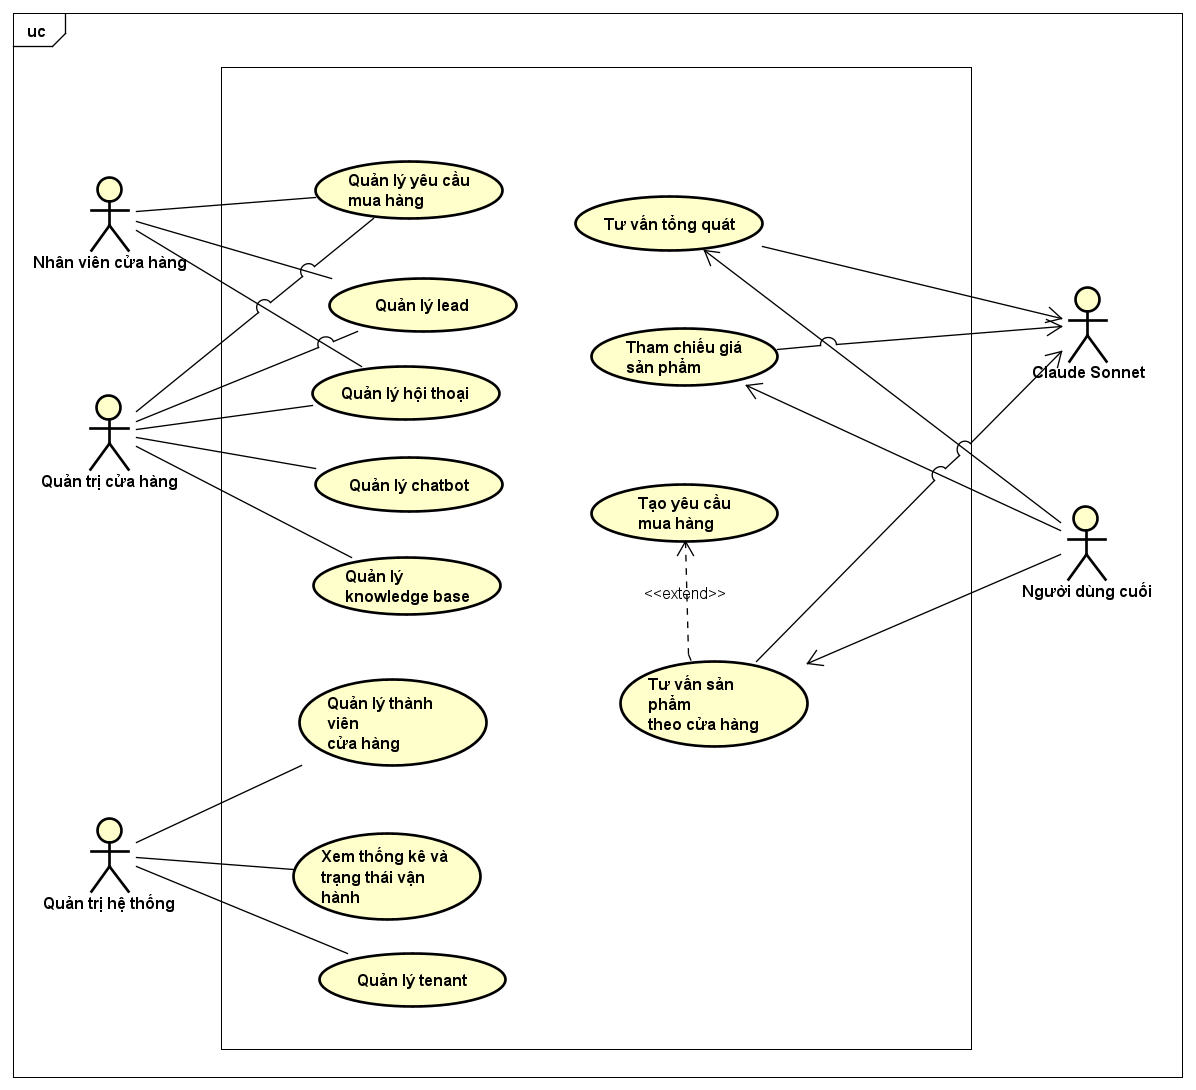
\includegraphics[width=0.95\textwidth]{../Hinhve/Hinh2_1_usecase_tong_quat.png}
    \caption{Biểu đồ use case tổng quát của hệ thống}
    \label{fig:usecase-tong-quat}
\end{figure}

Trong hệ thống, người dùng cuối là tác nhân sử dụng các chức năng phục vụ quá trình tìm hiểu và lựa chọn sản phẩm nội thất. Tác nhân này có thể thực hiện các use case như tư vấn sản phẩm theo cửa hàng, tư vấn tổng quát, tham chiếu giá cơ bản và tạo yêu cầu mua hàng. Các chức năng này phản ánh quá trình người dùng trao đổi với chatbot để tìm sản phẩm phù hợp, hỏi thêm thông tin liên quan đến sản phẩm hoặc giá và gửi thông tin nhu cầu khi muốn được cửa hàng tiếp tục xử lý.

Nhân viên cửa hàng là tác nhân trực tiếp xử lý các thông tin phát sinh từ quá trình tư vấn. Tác nhân này có thể xem hội thoại, xem lead, phản hồi lead, claim yêu cầu mua hàng và cập nhật trạng thái xử lý. Nhân viên cửa hàng không quản lý toàn bộ cấu hình hệ thống, mà tập trung vào các nghiệp vụ phát sinh sau khi khách hàng tương tác với chatbot.

Quản trị cửa hàng là tác nhân chịu trách nhiệm vận hành chatbot của một tenant. Tác nhân này có thể quản lý chatbot, quản lý nguồn dữ liệu knowledge base, theo dõi trạng thái rebuild, xem hội thoại, quản lý lead và quản lý yêu cầu mua hàng trong phạm vi cửa hàng của mình. Vai trò này giúp cửa hàng chủ động cập nhật dữ liệu và theo dõi quá trình tư vấn của chatbot.

Quản trị hệ thống là tác nhân chịu trách nhiệm quản lý các thành phần chung của nền tảng. Tác nhân này có thể quản lý tenant, quản lý thành viên cửa hàng và theo dõi thống kê hoặc trạng thái vận hành chung. Nhóm chức năng này cần thiết vì hệ thống được xây dựng theo mô hình nhiều tenant, trong đó nhiều cửa hàng cùng sử dụng một nền tảng nhưng dữ liệu và cấu hình cần được tách biệt.

Các use case mức cao trong biểu đồ tổng quát gồm tư vấn sản phẩm theo cửa hàng, tư vấn tổng quát, tạo yêu cầu mua hàng, tham chiếu giá cơ bản, quản lý chatbot, quản lý knowledge base, quản lý hội thoại, quản lý lead, quản lý yêu cầu mua hàng, quản lý tenant, quản lý thành viên cửa hàng, xem thống kê và trạng thái vận hành, tích hợp Messenger và tích hợp Telegram. Trong các phần tiếp theo, một số use case mức cao có vai trò quan trọng sẽ được phân rã để làm rõ các chức năng con bên trong.

\subsection{Biểu đồ use case phân rã Tư vấn sản phẩm theo cửa hàng}
\label{subsection:2.2.2}

Use case tư vấn sản phẩm theo cửa hàng mô tả nhóm chức năng phục vụ người dùng cuối khi trao đổi với chatbot của một cửa hàng cụ thể. Đây là nhóm chức năng cốt lõi của hệ thống, vì nó gắn trực tiếp với mục tiêu hỗ trợ tư vấn bán hàng nội thất dựa trên dữ liệu riêng của từng cửa hàng. Biểu đồ phân rã use case này được trình bày trong Hình~\ref{fig:usecase-tu-van-san-pham}.

\begin{figure}[H]
    \centering
    % TODO: Chèn sơ đồ use case phân rã Tư vấn sản phẩm theo cửa hàng tại đây.
    % \includegraphics[width=0.95\textwidth]{figures/usecase-tu-van-san-pham.pdf}
    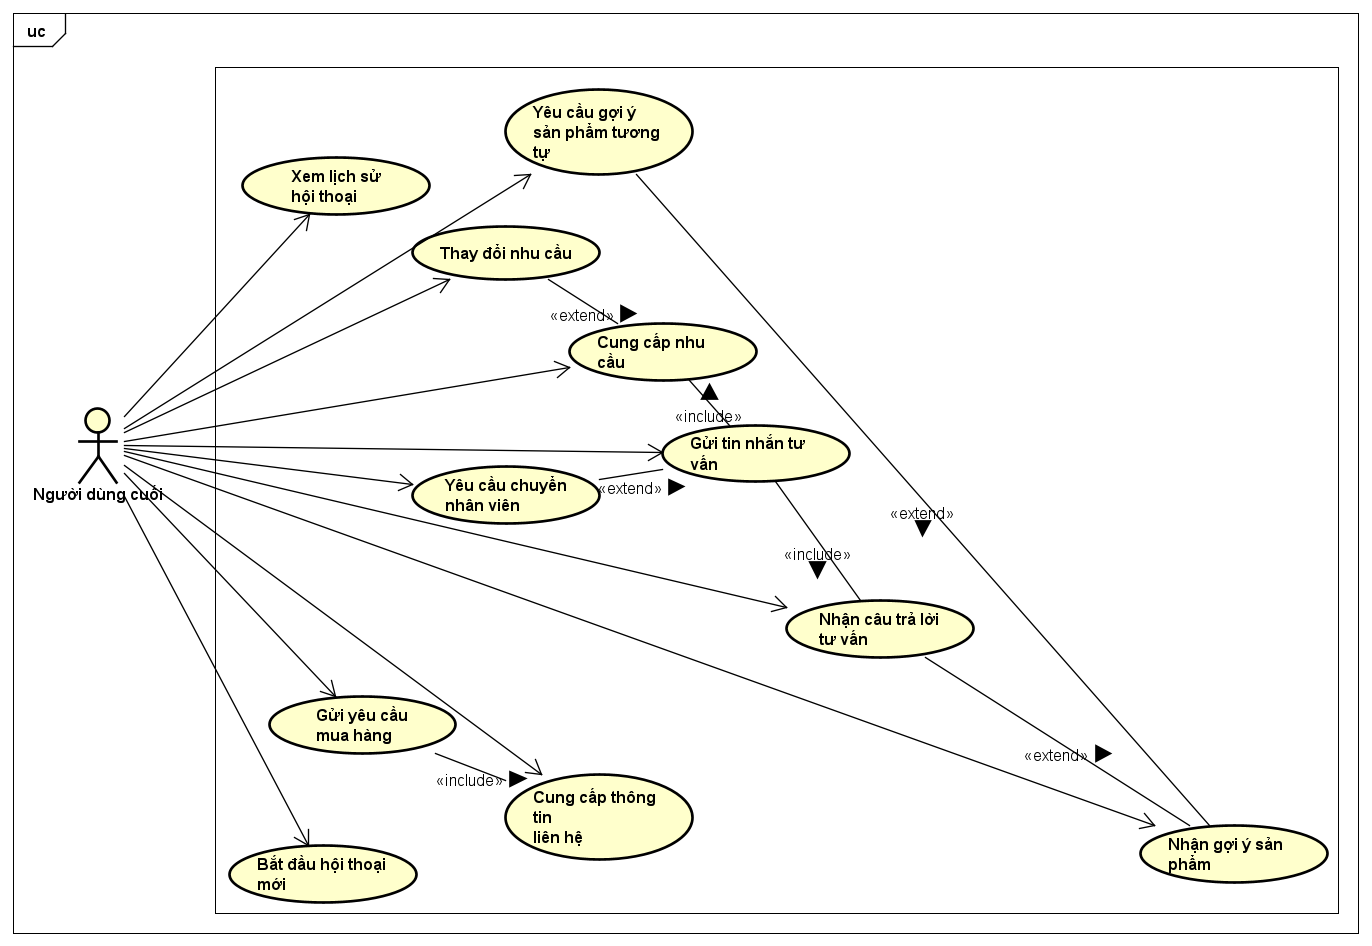
\includegraphics[width=0.95\textwidth]{../Hinhve/Hinh2_2_usecase_tu_van_san_pham.png}
    \caption{Biểu đồ use case phân rã Tư vấn sản phẩm theo cửa hàng}
    \label{fig:usecase-tu-van-san-pham}
\end{figure}

Trong nhóm chức năng này, người dùng cuối bắt đầu bằng việc mở giao diện chat của một cửa hàng và gửi yêu cầu tư vấn cho chatbot. Yêu cầu có thể liên quan đến loại sản phẩm, ngân sách, kích thước, chất liệu, phong cách hoặc bối cảnh sử dụng. Sau khi tiếp nhận yêu cầu, hệ thống xử lý nội dung hội thoại, truy xuất thông tin liên quan từ knowledge base của cửa hàng và trả về câu trả lời tư vấn phù hợp.

Use case tư vấn sản phẩm theo cửa hàng có thể được phân rã thành các use case con gồm bắt đầu hội thoại mới, gửi tin nhắn tư vấn, cung cấp nhu cầu, thay đổi nhu cầu, nhận câu trả lời tư vấn, nhận gợi ý sản phẩm, yêu cầu gợi ý sản phẩm tương tự, xem lịch sử hội thoại, gửi yêu cầu mua hàng, cung cấp thông tin liên hệ và yêu cầu chuyển nhân viên. Trong quá trình hội thoại, người dùng không bị giới hạn ở một lượt hỏi đáp cố định mà có thể tiếp tục bổ sung hoặc điều chỉnh nhu cầu. Ví dụ, người dùng có thể thay đổi ngân sách, yêu cầu sản phẩm có chất liệu khác hoặc từ chối gợi ý trước đó để nhận một phương án phù hợp hơn.

Chức năng nhận gợi ý sản phẩm cho phép người dùng xem các sản phẩm được hệ thống đề xuất dựa trên nội dung đã trao đổi. Khi người dùng đã có nhu cầu rõ ràng hơn, chức năng gửi yêu cầu mua hàng được sử dụng để ghi nhận thông tin khách hàng, sản phẩm quan tâm và nội dung tư vấn liên quan. Yêu cầu này sau đó được chuyển sang nhóm chức năng quản lý lead hoặc quản lý yêu cầu mua hàng để cửa hàng tiếp tục xử lý.

\subsection{Biểu đồ use case phân rã Quản lý chatbot và knowledge base}
\label{subsection:2.2.3}

Use case quản lý chatbot và knowledge base mô tả nhóm chức năng dành cho quản trị cửa hàng trong quá trình chuẩn bị và vận hành chatbot. Nhóm chức năng này cho phép mỗi cửa hàng quản lý chatbot và nguồn dữ liệu phục vụ tư vấn trong phạm vi tenant của mình. Biểu đồ phân rã use case quản lý chatbot và knowledge base được trình bày trong Hình~\ref{fig:usecase-quan-ly-chatbot-kb}.

\begin{figure}[H]
    \centering
    % TODO: Chèn sơ đồ use case phân rã Quản lý chatbot và knowledge base tại đây.
    % \includegraphics[width=0.95\textwidth]{figures/usecase-quan-ly-chatbot-kb.pdf}
    
\includegraphics[width=0.95\textwidth]{../Hinhve/Hinh2_3_usecase_quan_ly_chatbot_kb.png}
    \caption{Biểu đồ use case phân rã Quản lý chatbot và knowledge base}
    \label{fig:usecase-quan-ly-chatbot-kb}
\end{figure}

Trong nhóm chức năng này, quản trị cửa hàng có thể thực hiện các thao tác liên quan đến chatbot như tạo chatbot, xem danh sách chatbot và cập nhật cấu hình chatbot. Các thao tác này giúp cửa hàng thiết lập chatbot phù hợp với mục đích tư vấn, kênh sử dụng và phong cách phản hồi mong muốn.

Bên cạnh chatbot, cửa hàng cần quản lý knowledge base dùng làm nguồn dữ liệu cho quá trình tư vấn. Các use case con liên quan đến knowledge base gồm xem danh sách nguồn dữ liệu, thêm nguồn dữ liệu vào knowledge base, xóa nguồn dữ liệu khỏi knowledge base, rebuild knowledge base, xem trạng thái knowledge base và xem lịch sử rebuild. Dữ liệu trong knowledge base có thể bao gồm thông tin sản phẩm hoặc tài liệu liên quan đến sản phẩm của cửa hàng. Việc quản lý knowledge base là cần thiết vì chất lượng tư vấn của chatbot phụ thuộc trực tiếp vào dữ liệu mà hệ thống có thể truy xuất.

Quản trị hệ thống có thể theo dõi trạng thái knowledge base của các tenant ở mức tổng quan để phục vụ vận hành. Tuy nhiên, các thao tác cập nhật dữ liệu cụ thể vẫn thuộc phạm vi của quản trị cửa hàng. Nhóm chức năng này không đi sâu vào cách dữ liệu được xử lý ở tầng kỹ thuật, mà tập trung vào các thao tác nghiệp vụ mà cửa hàng cần thực hiện.

\subsection{Biểu đồ use case phân rã Quản lý hội thoại và yêu cầu mua hàng}
\label{subsection:2.2.4}

Use case quản lý hội thoại và yêu cầu mua hàng mô tả nhóm chức năng dành cho nhân viên cửa hàng và quản trị cửa hàng sau khi người dùng đã tương tác với chatbot. Nhóm chức năng này giúp cửa hàng theo dõi quá trình tư vấn, xử lý lead và tiếp nhận các yêu cầu mua hàng được tạo ra từ hội thoại. Biểu đồ phân rã use case này được trình bày trong Hình~\ref{fig:usecase-quan-ly-hoi-thoai-yeu-cau}.

\begin{figure}[H]
    \centering
    % TODO: Chèn sơ đồ use case phân rã Quản lý hội thoại và yêu cầu mua hàng tại đây.
    % \includegraphics[width=0.95\textwidth]{figures/usecase-quan-ly-hoi-thoai-yeu-cau.pdf}
    
\includegraphics[width=0.95\textwidth]{../Hinhve/Hinh2_4_usecase_quan_ly_hoi_thoai_yeu_cau.png}
    \caption{Biểu đồ use case phân rã Quản lý hội thoại và yêu cầu mua hàng}
    \label{fig:usecase-quan-ly-hoi-thoai-yeu-cau}
\end{figure}

Đối với quản lý hội thoại, nhân viên cửa hàng có thể xem danh sách hội thoại, lọc hội thoại và xem chi tiết từng hội thoại giữa người dùng với chatbot. Chức năng này giúp cửa hàng nắm được nội dung người dùng đã trao đổi, các nhu cầu đã được ghi nhận và các sản phẩm đã được tư vấn. Việc theo dõi hội thoại cũng hỗ trợ cửa hàng đánh giá chất lượng tư vấn và tiếp tục xử lý trong trường hợp cần nhân viên can thiệp.

Đối với quản lý lead, nhân viên cửa hàng có thể xem danh sách lead, xem chi tiết lead, cập nhật trạng thái lead và phản hồi lead qua kênh chat nếu kênh tương ứng đã được cấu hình. Lead là thông tin khách hàng tiềm năng được tạo từ hội thoại khi người dùng thể hiện nhu cầu mua hàng hoặc để lại thông tin liên hệ. Việc quản lý lead giúp cửa hàng không bỏ sót các cơ hội bán hàng phát sinh từ chatbot.

Đối với quản lý yêu cầu mua hàng, nhân viên cửa hàng có thể xem danh sách yêu cầu mua hàng, lọc yêu cầu theo trạng thái, claim yêu cầu mua hàng và cập nhật trạng thái xử lý. Quản trị cửa hàng có thêm quyền phân công lại yêu cầu mua hàng cho nhân viên khác khi cần. Một yêu cầu mua hàng có thể bao gồm thông tin người dùng, sản phẩm quan tâm, ghi chú và nội dung liên quan đến quá trình tư vấn. Nhóm use case này có quan hệ trực tiếp với use case tư vấn sản phẩm theo cửa hàng, vì kết quả của một phiên tư vấn có thể được chuyển thành lead hoặc yêu cầu mua hàng để cửa hàng tiếp tục xử lý.

\subsection{Biểu đồ use case phân rã Tham chiếu giá cơ bản}
\label{subsection:2.2.5}

Use case tham chiếu giá cơ bản mô tả nhóm chức năng phục vụ người dùng cuối khi cần tham khảo khoảng giá của một loại sản phẩm hoặc đánh giá một mức giá cụ thể so với dữ liệu tham chiếu trong phạm vi hệ thống. Chức năng này không nhằm định giá toàn bộ thị trường nội thất, mà chỉ cung cấp thông tin tham khảo ban đầu dựa trên dữ liệu hệ thống có sẵn. Biểu đồ phân rã use case này được trình bày trong Hình~\ref{fig:usecase-tham-chieu-gia-co-ban}.

\begin{figure}[H]
    \centering
    % TODO: Chèn sơ đồ use case phân rã Tham chiếu giá cơ bản tại đây.
    % \includegraphics[width=0.95\textwidth]{figures/usecase-tham-chieu-gia-co-ban.pdf}
    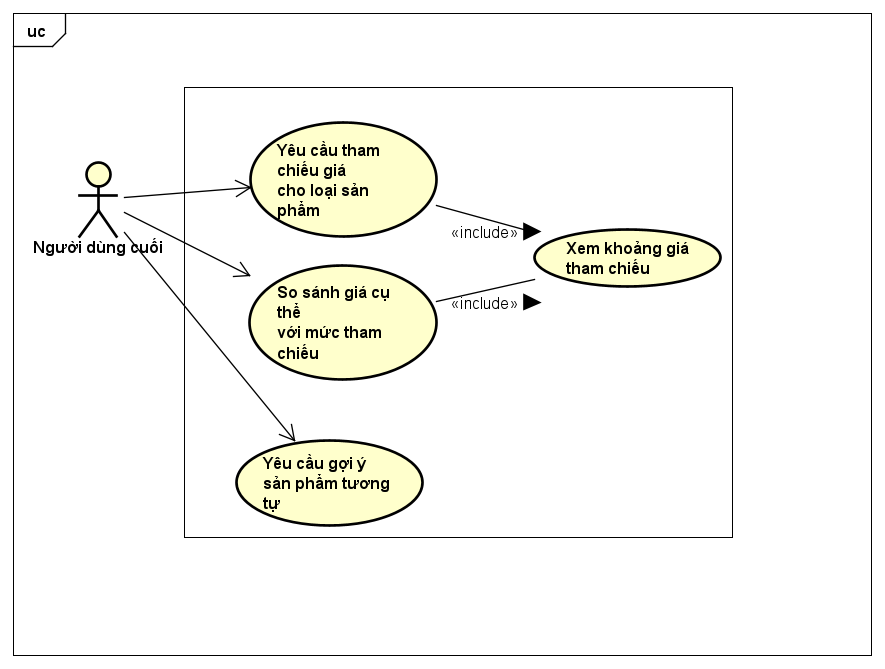
\includegraphics[width=0.95\textwidth]{../Hinhve/Hinh2_5_usecase_tham_chieu_gia_co_ban.png}
    \caption{Biểu đồ use case phân rã Tham chiếu giá cơ bản}
    \label{fig:usecase-tham-chieu-gia-co-ban}
\end{figure}

Các use case con trong nhóm này gồm yêu cầu tham chiếu giá cho loại sản phẩm, xem khoảng giá tham chiếu, so sánh một mức giá cụ thể với khoảng tham chiếu và yêu cầu gợi ý sản phẩm tương tự nếu phù hợp. Khi hệ thống không xác định được loại sản phẩm hoặc chưa có dữ liệu tham chiếu tương ứng, chatbot cần yêu cầu người dùng làm rõ hoặc thông báo rằng chưa có đủ dữ liệu để đưa ra nhận xét.

Chức năng tham chiếu giá cơ bản giúp người dùng có thêm thông tin trước khi ra quyết định, đặc biệt trong các tình huống người dùng chưa rõ mức giá của một nhóm sản phẩm hoặc muốn biết một mức giá cụ thể có nằm trong khoảng tham chiếu hay không. Tuy nhiên, kết quả trả về chỉ có ý nghĩa trong phạm vi dữ liệu được hệ thống quản lý, không thay thế cho khảo sát thị trường đầy đủ hoặc báo giá chính thức từ cửa hàng.

\subsection{Quy trình nghiệp vụ}
\label{subsection:2.2.6}

Bên cạnh các use case riêng lẻ, hệ thống có một số quy trình nghiệp vụ kết hợp nhiều chức năng. Các quy trình này giúp mô tả cách hệ thống được sử dụng trong thực tế, từ lúc cửa hàng cấu hình chatbot, người dùng chat tư vấn, đến khi nhân viên cửa hàng xử lý lead hoặc yêu cầu mua hàng.

\subsubsection{Quy trình cửa hàng cấu hình chatbot và xây dựng knowledge base}

Quy trình này mô tả các bước cửa hàng thực hiện để chuẩn bị chatbot trước khi đưa vào sử dụng. Quản trị cửa hàng đăng nhập vào hệ thống, tạo hoặc cập nhật chatbot, thêm nguồn dữ liệu cho knowledge base, kích hoạt rebuild và kiểm tra trạng thái xử lý. Khi knowledge base đã sẵn sàng, chatbot có thể sử dụng dữ liệu đó để tư vấn cho người dùng cuối.

\begin{figure}[H]
    \centering
    % TODO: Chèn activity diagram quy trình cấu hình chatbot và xây dựng knowledge base tại đây.
    % \includegraphics[width=0.95\textwidth]{figures/activity-cau-hinh-chatbot-kb.pdf}
    
\includegraphics[width=0.95\textwidth]{../Hinhve/Hinh2_6_activity_cau_hinh_chatbot_kb.png}
    \caption{Biểu đồ hoạt động quy trình cửa hàng cấu hình chatbot và xây dựng knowledge base}
    \label{fig:activity-cau-hinh-chatbot-kb}
\end{figure}

Quy trình bắt đầu khi quản trị cửa hàng đăng nhập vào hệ thống và truy cập trang quản lý chatbot. Nếu cửa hàng chưa có chatbot, quản trị cửa hàng tạo chatbot mới; nếu đã có chatbot, quản trị cửa hàng có thể cập nhật cấu hình phù hợp với nhu cầu tư vấn. Sau đó, quản trị cửa hàng chuyển sang phần quản lý knowledge base, thêm hoặc cập nhật nguồn dữ liệu và kích hoạt rebuild. Hệ thống xử lý dữ liệu, cập nhật trạng thái knowledge base và thông báo kết quả cho quản trị cửa hàng.

\subsubsection{Quy trình khách hàng chat tư vấn và tạo yêu cầu mua hàng}

Quy trình này mô tả luồng người dùng cuối trao đổi với chatbot của một cửa hàng. Người dùng bắt đầu hội thoại, nhập nhu cầu, nhận tư vấn và có thể tiếp tục điều chỉnh yêu cầu. Khi người dùng thể hiện ý định mua hàng và cung cấp đủ thông tin cần thiết, hệ thống tạo lead hoặc yêu cầu mua hàng để cửa hàng tiếp tục xử lý.

\begin{figure}[H]
    \centering
    % TODO: Chèn activity diagram quy trình khách hàng chat tư vấn và tạo yêu cầu mua hàng tại đây.
    % \includegraphics[width=0.95\textwidth]{figures/activity-chat-tu-van-tao-yeu-cau.pdf}
    
\includegraphics[width=0.95\textwidth]{../Hinhve/Hinh2_7_activity_chat_tu_van_tao_yeu_cau.png}
    \caption{Biểu đồ hoạt động quy trình khách hàng chat tư vấn và tạo yêu cầu mua hàng}
    \label{fig:activity-chat-tu-van-tao-yeu-cau}
\end{figure}

Quy trình bắt đầu khi người dùng mở giao diện chat và nhập nhu cầu tư vấn. Hệ thống tiếp nhận nội dung, xác định ngữ cảnh hội thoại, truy xuất dữ liệu phù hợp từ knowledge base và trả về câu trả lời tư vấn. Nếu người dùng tiếp tục trao đổi, hệ thống cập nhật ngữ cảnh và xử lý các yêu cầu tiếp theo. Khi người dùng muốn mua hàng, chatbot thu thập thông tin liên hệ hoặc thông tin sản phẩm quan tâm, sau đó hệ thống tạo lead hoặc yêu cầu mua hàng để cửa hàng tiếp nhận.

\subsubsection{Quy trình nhân viên cửa hàng xử lý lead/yêu cầu mua hàng}

Quy trình này mô tả cách nhân viên cửa hàng xử lý thông tin sau khi hệ thống tạo lead hoặc yêu cầu mua hàng từ hội thoại. Nhân viên xem danh sách yêu cầu, kiểm tra nội dung hội thoại, claim yêu cầu nếu cần, liên hệ khách hàng và cập nhật trạng thái xử lý.

\begin{figure}[H]
    \centering
    % TODO: Chèn activity diagram quy trình nhân viên cửa hàng xử lý lead/yêu cầu mua hàng tại đây.
    % \includegraphics[width=0.95\textwidth]{figures/activity-xu-ly-lead-yeu-cau.pdf}
    
\includegraphics[width=0.95\textwidth]{../Hinhve/Hinh2_8_activity_xu_ly_lead_yeu_cau.png}
    \caption{Biểu đồ hoạt động quy trình nhân viên cửa hàng xử lý lead/yêu cầu mua hàng}
    \label{fig:activity-xu-ly-lead-yeu-cau}
\end{figure}

Quy trình bắt đầu khi nhân viên cửa hàng đăng nhập và truy cập danh sách lead hoặc yêu cầu mua hàng. Nhân viên chọn một bản ghi cần xử lý, xem chi tiết nhu cầu và lịch sử hội thoại, sau đó claim yêu cầu nếu chưa có người xử lý. Tiếp theo, nhân viên liên hệ hoặc phản hồi khách hàng, cập nhật trạng thái xử lý và đánh dấu hoàn thành nếu yêu cầu đã được xử lý xong. Trong trường hợp cần điều phối lại, quản trị cửa hàng có thể phân công lại yêu cầu cho nhân viên khác.

\section{Đặc tả chức năng}
\label{section:2.3}

Trong phần này, đồ án lựa chọn sáu use case quan trọng để đặc tả chi tiết. Các use case được chọn gồm quản lý chatbot, quản lý nguồn dữ liệu knowledge base, rebuild knowledge base, tư vấn sản phẩm theo cửa hàng, tạo yêu cầu mua hàng từ hội thoại và quản lý yêu cầu mua hàng. Đây là các use case đại diện cho luồng vận hành chính của hệ thống, từ chuẩn bị dữ liệu, vận hành chatbot đến xử lý thông tin mua hàng phát sinh từ hội thoại.

\subsection{Đặc tả use case UC0004: Quản lý chatbot}
\label{subsection:2.3.1}

\begin{table}[H]
\centering
\caption{Bảng đặc tả use case UC0004}
\label{table:uc0004}
\begin{tabular}{|p{0.28\textwidth}|p{0.62\textwidth}|}
\hline
\textbf{Thuộc tính} & \textbf{Mô tả} \\
\hline
Mã use case & UC0004 \\
\hline
Tên use case & Quản lý chatbot \\
\hline
Tác nhân & Quản trị cửa hàng \\
\hline
Mục tiêu & Tạo và cấu hình chatbot phục vụ tư vấn cho cửa hàng \\
\hline
Tiền điều kiện & Quản trị cửa hàng đã đăng nhập và có quyền quản lý chatbot trong tenant của mình \\
\hline
Hậu điều kiện & Chatbot được tạo mới hoặc cấu hình chatbot hiện có được cập nhật \\
\hline
\end{tabular}
\end{table}

\textbf{Luồng sự kiện chính}

\begin{table}[H]
\centering
\begin{tabular}{|p{0.08\textwidth}|p{0.22\textwidth}|p{0.60\textwidth}|}
\hline
\textbf{STT} & \textbf{Thực hiện} & \textbf{Hành động} \\
\hline
1 & Quản trị cửa hàng & Mở màn hình quản lý chatbot. \\
\hline
2 & Hệ thống & Hiển thị danh sách chatbot thuộc tenant hiện tại. \\
\hline
3 & Quản trị cửa hàng & Chọn tạo chatbot mới hoặc cập nhật chatbot hiện có. \\
\hline
4 & Quản trị cửa hàng & Nhập tên chatbot, kênh sử dụng, persona, chế độ hoạt động và các thông tin cấu hình liên quan. \\
\hline
5 & Hệ thống & Kiểm tra dữ liệu đầu vào và quyền thao tác. \\
\hline
6 & Hệ thống & Lưu thông tin chatbot. \\
\hline
7 & Hệ thống & Hiển thị kết quả thao tác và cập nhật danh sách chatbot. \\
\hline
\end{tabular}
\end{table}

\textbf{Luồng sự kiện thay thế}

\begin{table}[H]
\centering
\begin{tabular}{|p{0.08\textwidth}|p{0.22\textwidth}|p{0.60\textwidth}|}
\hline
\textbf{STT} & \textbf{Thực hiện} & \textbf{Hành động} \\
\hline
5.1 & Hệ thống & Thông báo lỗi nếu thiếu trường bắt buộc hoặc dữ liệu không hợp lệ. \\
\hline
5.2 & Hệ thống & Từ chối thao tác nếu người dùng không thuộc tenant tương ứng hoặc không có quyền quản lý chatbot. \\
\hline
6.1 & Hệ thống & Thông báo lưu cấu hình thất bại nếu có lỗi trong quá trình xử lý. \\
\hline
\end{tabular}
\end{table}

\subsection{Đặc tả use case UC0005: Quản lý nguồn dữ liệu knowledge base}
\label{subsection:2.3.2}

\begin{table}[H]
\centering
\caption{Bảng đặc tả use case UC0005}
\label{table:uc0005}
\begin{tabular}{|p{0.28\textwidth}|p{0.62\textwidth}|}
\hline
\textbf{Thuộc tính} & \textbf{Mô tả} \\
\hline
Mã use case & UC0005 \\
\hline
Tên use case & Quản lý nguồn dữ liệu knowledge base \\
\hline
Tác nhân & Quản trị cửa hàng \\
\hline
Mục tiêu & Quản lý các nguồn dữ liệu dùng để xây dựng knowledge base của cửa hàng \\
\hline
Tiền điều kiện & Quản trị cửa hàng đã đăng nhập và có quyền quản lý dữ liệu của tenant \\
\hline
Hậu điều kiện & Danh sách nguồn dữ liệu knowledge base được cập nhật \\
\hline
\end{tabular}
\end{table}

\textbf{Luồng sự kiện chính}

\begin{table}[H]
\centering
\begin{tabular}{|p{0.08\textwidth}|p{0.22\textwidth}|p{0.60\textwidth}|}
\hline
\textbf{STT} & \textbf{Thực hiện} & \textbf{Hành động} \\
\hline
1 & Quản trị cửa hàng & Mở màn hình quản lý knowledge base. \\
\hline
2 & Hệ thống & Hiển thị danh sách nguồn dữ liệu hiện có của tenant. \\
\hline
3 & Quản trị cửa hàng & Thêm mới, kiểm tra hoặc xóa nguồn dữ liệu. \\
\hline
4 & Hệ thống & Kiểm tra định dạng và tính hợp lệ của nguồn dữ liệu. \\
\hline
5 & Hệ thống & Lưu thay đổi vào hệ thống. \\
\hline
6 & Hệ thống & Hiển thị danh sách nguồn dữ liệu sau khi cập nhật. \\
\hline
\end{tabular}
\end{table}

\textbf{Luồng sự kiện thay thế}

\begin{table}[H]
\centering
\begin{tabular}{|p{0.08\textwidth}|p{0.22\textwidth}|p{0.60\textwidth}|}
\hline
\textbf{STT} & \textbf{Thực hiện} & \textbf{Hành động} \\
\hline
4.1 & Hệ thống & Thông báo nguồn dữ liệu không hợp lệ hoặc không thể truy cập. \\
\hline
5.1 & Hệ thống & Thông báo lưu thay đổi thất bại. \\
\hline
5.2 & Hệ thống & Từ chối thao tác nếu người dùng không có quyền trên tenant tương ứng. \\
\hline
\end{tabular}
\end{table}

\subsection{Đặc tả use case UC0006: Rebuild knowledge base}
\label{subsection:2.3.3}

\begin{table}[H]
\centering
\caption{Bảng đặc tả use case UC0006}
\label{table:uc0006}
\begin{tabular}{|p{0.28\textwidth}|p{0.62\textwidth}|}
\hline
\textbf{Thuộc tính} & \textbf{Mô tả} \\
\hline
Mã use case & UC0006 \\
\hline
Tên use case & Rebuild knowledge base \\
\hline
Tác nhân & Quản trị cửa hàng \\
\hline
Mục tiêu & Xử lý lại nguồn dữ liệu để cập nhật knowledge base phục vụ tư vấn \\
\hline
Tiền điều kiện & Cửa hàng đã có ít nhất một nguồn dữ liệu hợp lệ \\
\hline
Hậu điều kiện & Knowledge base được build lại hoặc hệ thống ghi nhận lỗi xử lý \\
\hline
\end{tabular}
\end{table}

\textbf{Luồng sự kiện chính}

\begin{table}[H]
\centering
\begin{tabular}{|p{0.08\textwidth}|p{0.22\textwidth}|p{0.60\textwidth}|}
\hline
\textbf{STT} & \textbf{Thực hiện} & \textbf{Hành động} \\
\hline
1 & Quản trị cửa hàng & Chọn chức năng rebuild knowledge base. \\
\hline
2 & Hệ thống & Kiểm tra danh sách nguồn dữ liệu của tenant. \\
\hline
3 & Hệ thống & Thu thập và xử lý dữ liệu từ các nguồn đã cấu hình. \\
\hline
4 & Hệ thống & Tạo lại dữ liệu phục vụ truy xuất cho chatbot. \\
\hline
5 & Hệ thống & Cập nhật trạng thái knowledge base. \\
\hline
6 & Quản trị cửa hàng & Xem kết quả rebuild và lịch sử xử lý. \\
\hline
\end{tabular}
\end{table}

\textbf{Luồng sự kiện thay thế}

\begin{table}[H]
\centering
\begin{tabular}{|p{0.08\textwidth}|p{0.22\textwidth}|p{0.60\textwidth}|}
\hline
\textbf{STT} & \textbf{Thực hiện} & \textbf{Hành động} \\
\hline
2.1 & Hệ thống & Thông báo chưa có nguồn dữ liệu hợp lệ để rebuild. \\
\hline
3.1 & Hệ thống & Ghi nhận lỗi nếu không truy cập được nguồn dữ liệu. \\
\hline
4.1 & Hệ thống & Ghi nhận lỗi nếu quá trình xử lý dữ liệu thất bại. \\
\hline
5.1 & Hệ thống & Cập nhật trạng thái rebuild thất bại và hiển thị thông báo lỗi. \\
\hline
\end{tabular}
\end{table}

\subsection{Đặc tả use case UC0007: Tư vấn sản phẩm theo cửa hàng}
\label{subsection:2.3.4}

\begin{table}[H]
\centering
\caption{Bảng đặc tả use case UC0007}
\label{table:uc0007}
\begin{tabular}{|p{0.28\textwidth}|p{0.62\textwidth}|}
\hline
\textbf{Thuộc tính} & \textbf{Mô tả} \\
\hline
Mã use case & UC0007 \\
\hline
Tên use case & Tư vấn sản phẩm theo cửa hàng \\
\hline
Tác nhân & Người dùng cuối \\
\hline
Mục tiêu & Hỗ trợ người dùng tìm và đánh giá sản phẩm nội thất dựa trên dữ liệu của một cửa hàng cụ thể \\
\hline
Tiền điều kiện & Chatbot của cửa hàng đã được cấu hình và có knowledge base khả dụng \\
\hline
Hậu điều kiện & Câu trả lời tư vấn được hiển thị và nội dung hội thoại được lưu lại \\
\hline
\end{tabular}
\end{table}

\textbf{Luồng sự kiện chính}

\begin{table}[H]
\centering
\begin{tabular}{|p{0.08\textwidth}|p{0.22\textwidth}|p{0.60\textwidth}|}
\hline
\textbf{STT} & \textbf{Thực hiện} & \textbf{Hành động} \\
\hline
1 & Người dùng cuối & Mở giao diện chat của cửa hàng. \\
\hline
2 & Người dùng cuối & Bắt đầu hội thoại mới hoặc tiếp tục hội thoại đã có. \\
\hline
3 & Người dùng cuối & Nhập nhu cầu tư vấn bằng ngôn ngữ tự nhiên. \\
\hline
4 & Hệ thống & Tiếp nhận câu hỏi và xác định ngữ cảnh hội thoại. \\
\hline
5 & Hệ thống & Truy xuất dữ liệu liên quan từ knowledge base của cửa hàng. \\
\hline
6 & Hệ thống & Sinh câu trả lời tư vấn và gợi ý sản phẩm phù hợp nếu có. \\
\hline
7 & Hệ thống & Hiển thị câu trả lời cho người dùng. \\
\hline
8 & Hệ thống & Lưu nội dung hội thoại. \\
\hline
\end{tabular}
\end{table}

\textbf{Luồng sự kiện thay thế}

\begin{table}[H]
\centering
\begin{tabular}{|p{0.08\textwidth}|p{0.22\textwidth}|p{0.60\textwidth}|}
\hline
\textbf{STT} & \textbf{Thực hiện} & \textbf{Hành động} \\
\hline
3.1 & Người dùng cuối & Thay đổi nhu cầu, ngân sách hoặc tiêu chí sản phẩm trong quá trình trao đổi. \\
\hline
5.1 & Hệ thống & Thông báo chưa tìm được dữ liệu phù hợp trong knowledge base. \\
\hline
6.1 & Hệ thống & Yêu cầu người dùng bổ sung thông tin khi nhu cầu chưa rõ. \\
\hline
7.1 & Người dùng cuối & Yêu cầu chuyển cho nhân viên tư vấn nếu muốn được cửa hàng hỗ trợ trực tiếp. \\
\hline
\end{tabular}
\end{table}

\subsection{Đặc tả use case UC0009: Tạo yêu cầu mua hàng từ hội thoại}
\label{subsection:2.3.5}

\begin{table}[H]
\centering
\caption{Bảng đặc tả use case UC0009}
\label{table:uc0009}
\begin{tabular}{|p{0.28\textwidth}|p{0.62\textwidth}|}
\hline
\textbf{Thuộc tính} & \textbf{Mô tả} \\
\hline
Mã use case & UC0009 \\
\hline
Tên use case & Tạo yêu cầu mua hàng từ hội thoại \\
\hline
Tác nhân & Người dùng cuối, hệ thống \\
\hline
Mục tiêu & Ghi nhận nhu cầu mua hàng của người dùng để cửa hàng tiếp tục xử lý \\
\hline
Tiền điều kiện & Người dùng đang trong hội thoại tư vấn theo cửa hàng \\
\hline
Hậu điều kiện & Lead hoặc yêu cầu mua hàng được tạo và gắn với hội thoại tương ứng \\
\hline
\end{tabular}
\end{table}

\textbf{Luồng sự kiện chính}

\begin{table}[H]
\centering
\begin{tabular}{|p{0.08\textwidth}|p{0.22\textwidth}|p{0.60\textwidth}|}
\hline
\textbf{STT} & \textbf{Thực hiện} & \textbf{Hành động} \\
\hline
1 & Người dùng cuối & Thể hiện ý định mua hàng trong hội thoại. \\
\hline
2 & Hệ thống & Nhận diện ý định mua hàng từ nội dung hội thoại. \\
\hline
3 & Hệ thống & Yêu cầu hoặc trích xuất thông tin liên hệ cần thiết. \\
\hline
4 & Người dùng cuối & Cung cấp thông tin liên hệ, sản phẩm quan tâm hoặc ghi chú bổ sung nếu cần. \\
\hline
5 & Hệ thống & Tạo lead hoặc yêu cầu mua hàng từ hội thoại. \\
\hline
6 & Hệ thống & Thông báo cho người dùng rằng yêu cầu đã được ghi nhận. \\
\hline
\end{tabular}
\end{table}

\textbf{Luồng sự kiện thay thế}

\begin{table}[H]
\centering
\begin{tabular}{|p{0.08\textwidth}|p{0.22\textwidth}|p{0.60\textwidth}|}
\hline
\textbf{STT} & \textbf{Thực hiện} & \textbf{Hành động} \\
\hline
3.1 & Hệ thống & Yêu cầu bổ sung thông tin nếu dữ liệu còn thiếu. \\
\hline
5.1 & Hệ thống & Không tạo yêu cầu mới nếu hội thoại đã có yêu cầu mua hàng tương ứng trước đó. \\
\hline
5.2 & Hệ thống & Thông báo lỗi nếu lưu yêu cầu thất bại. \\
\hline
\end{tabular}
\end{table}

\subsection{Đặc tả use case UC0011: Quản lý yêu cầu mua hàng}
\label{subsection:2.3.6}

\begin{table}[H]
\centering
\caption{Bảng đặc tả use case UC0011}
\label{table:uc0011}
\begin{tabular}{|p{0.28\textwidth}|p{0.62\textwidth}|}
\hline
\textbf{Thuộc tính} & \textbf{Mô tả} \\
\hline
Mã use case & UC0011 \\
\hline
Tên use case & Quản lý yêu cầu mua hàng \\
\hline
Tác nhân & Nhân viên cửa hàng, quản trị cửa hàng \\
\hline
Mục tiêu & Tiếp nhận, phân công và cập nhật trạng thái yêu cầu mua hàng \\
\hline
Tiền điều kiện & Hệ thống đã có yêu cầu mua hàng phát sinh từ hội thoại \\
\hline
Hậu điều kiện & Yêu cầu mua hàng được cập nhật trạng thái hoặc phân công xử lý \\
\hline
\end{tabular}
\end{table}

\textbf{Luồng sự kiện chính}

\begin{table}[H]
\centering
\begin{tabular}{|p{0.08\textwidth}|p{0.22\textwidth}|p{0.60\textwidth}|}
\hline
\textbf{STT} & \textbf{Thực hiện} & \textbf{Hành động} \\
\hline
1 & Nhân viên cửa hàng & Mở danh sách yêu cầu mua hàng. \\
\hline
2 & Hệ thống & Hiển thị các yêu cầu thuộc tenant hiện tại. \\
\hline
3 & Nhân viên cửa hàng & Lọc hoặc chọn một yêu cầu để xử lý. \\
\hline
4 & Nhân viên cửa hàng & Claim yêu cầu nếu chưa có người xử lý. \\
\hline
5 & Nhân viên cửa hàng & Cập nhật trạng thái yêu cầu. \\
\hline
6 & Hệ thống & Lưu thay đổi và hiển thị kết quả. \\
\hline
\end{tabular}
\end{table}

\textbf{Luồng sự kiện thay thế}

\begin{table}[H]
\centering
\begin{tabular}{|p{0.08\textwidth}|p{0.22\textwidth}|p{0.60\textwidth}|}
\hline
\textbf{STT} & \textbf{Thực hiện} & \textbf{Hành động} \\
\hline
2.1 & Hệ thống & Hiển thị trạng thái trống nếu chưa có yêu cầu mua hàng. \\
\hline
4.1 & Hệ thống & Thông báo yêu cầu đã được người khác nhận xử lý. \\
\hline
5.1 & Quản trị cửa hàng & Phân công lại yêu cầu cho nhân viên khác nếu cần. \\
\hline
6.1 & Hệ thống & Thông báo cập nhật thất bại. \\
\hline
\end{tabular}
\end{table}

\section{Yêu cầu phi chức năng}
\label{section:2.4}

Bên cạnh các yêu cầu chức năng, hệ thống cần đáp ứng một số yêu cầu phi chức năng để đảm bảo khả năng vận hành, bảo trì và mở rộng trong phạm vi đồ án. Các yêu cầu này được chia thành các nhóm hiệu năng, độ tin cậy, bảo mật và phân quyền, tính dễ sử dụng, tính dễ bảo trì và khả năng mở rộng.

\subsection{Hiệu năng}

Hệ thống cần đảm bảo các trang quản trị như danh sách tenant, chatbot, lead và yêu cầu mua hàng được tải trong thời gian chấp nhận được với quy mô dữ liệu demo. Đối với chức năng chat, do quá trình xử lý có thể phụ thuộc vào AI service và truy xuất knowledge base, giao diện cần hiển thị trạng thái chờ trong khi hệ thống đang xử lý để người dùng biết yêu cầu đã được tiếp nhận. Đối với quy trình rebuild knowledge base, hệ thống cần ghi nhận trạng thái xử lý và không làm treo toàn bộ giao diện quản trị trong thời gian xử lý dữ liệu.

\subsection{Độ tin cậy}

Hệ thống cần lưu lại tin nhắn của người dùng và phản hồi của chatbot để phục vụ xem lại hội thoại, tạo lead hoặc tạo yêu cầu mua hàng. Khi người dùng đã tạo yêu cầu mua hàng từ một hội thoại, hệ thống cần hạn chế tạo lặp các bản ghi giống nhau nếu cùng một yêu cầu đã được ghi nhận trước đó. Đối với quá trình rebuild knowledge base, nếu có lỗi xảy ra, hệ thống cần lưu trạng thái lỗi để quản trị cửa hàng có thể kiểm tra. Khi AI service không phản hồi hoặc xảy ra lỗi trong quá trình xử lý, hệ thống cần thông báo phù hợp thay vì làm mất phiên hội thoại.

\subsection{Bảo mật và phân quyền}

Các chức năng quản trị cần yêu cầu đăng nhập. Hệ thống cần phân quyền theo vai trò, bao gồm quản trị hệ thống, quản trị cửa hàng và nhân viên cửa hàng. Quản trị hệ thống có quyền quản lý tenant và thành viên cửa hàng, trong khi quản trị cửa hàng và nhân viên cửa hàng chỉ được thao tác trên dữ liệu thuộc tenant của mình. Dữ liệu chatbot, knowledge base, hội thoại, lead và yêu cầu mua hàng của từng tenant cần được tách biệt. Các thông tin nhạy cảm như token tích hợp kênh chat ngoài hoặc khóa truy cập mô hình ngôn ngữ không được để lộ cho người dùng cuối.

\subsection{Tính dễ sử dụng}

Giao diện quản trị cần được tổ chức theo các nhóm chức năng rõ ràng như chatbot, knowledge base, hội thoại, lead và yêu cầu mua hàng. Các thao tác tạo, cập nhật, xóa hoặc rebuild cần có thông báo kết quả rõ ràng. Khi chatbot đang xử lý câu trả lời hoặc knowledge base đang được rebuild, giao diện cần hiển thị trạng thái chờ. Các thông báo lỗi cần được trình bày bằng ngôn ngữ dễ hiểu, giúp người dùng biết thao tác nào thất bại và cần xử lý ra sao.

\subsection{Tính dễ bảo trì}

Hệ thống cần tách rõ phần backend nghiệp vụ và phần AI service để dễ phát triển, kiểm thử và thay thế từng thành phần. Các thông số triển khai, endpoint, token và khóa truy cập dịch vụ ngoài cần được cấu hình bên ngoài mã nguồn khi có thể. Các dịch vụ chính cần ghi log để phục vụ theo dõi và chẩn đoán lỗi. API nên được tổ chức theo nhóm chức năng như chat, chatbot, knowledge base, tenant, lead, purchase request và vận hành hệ thống.

\subsection{Khả năng mở rộng}

Thiết kế hệ thống cần cho phép bổ sung tenant mới mà không phải tạo một hệ thống riêng cho từng cửa hàng. Hệ thống cũng cần có khả năng mở rộng thêm kênh chat ngoài khác trong tương lai nếu cần. AI service nên cho phép thay đổi mô hình ngôn ngữ hoặc provider ở mức cấu hình để phù hợp với điều kiện triển khai. Knowledge base của từng cửa hàng cần có khả năng bổ sung thêm nguồn dữ liệu mới khi danh mục sản phẩm hoặc tài liệu của cửa hàng thay đổi.

\section*{Kết chương}

Chương này đã trình bày quá trình khảo sát hiện trạng, phân tích nhu cầu của người dùng cuối, cửa hàng và quản trị hệ thống, đồng thời so sánh một số nhóm giải pháp hiện có liên quan đến chatbot tư vấn bán hàng. Từ kết quả khảo sát, chương đã xác định các nhóm chức năng chính của hệ thống multi-tenant RAG chatbot hỗ trợ tư vấn bán hàng nội thất, bao gồm tư vấn sản phẩm theo cửa hàng, quản lý chatbot và knowledge base, quản lý hội thoại, lead, yêu cầu mua hàng, tham chiếu giá cơ bản, tích hợp kênh chat ngoài và quản lý vận hành hệ thống.

Chương cũng đã mô tả các tác nhân tham gia hệ thống, các use case tổng quan và một số use case phân rã quan trọng. Bên cạnh đó, ba quy trình nghiệp vụ chính đã được trình bày để làm rõ cách hệ thống được sử dụng trong thực tế, từ cấu hình chatbot và knowledge base, chat tư vấn với khách hàng, đến xử lý lead và yêu cầu mua hàng. Cuối cùng, chương đã đặc tả sáu use case quan trọng và nêu các yêu cầu phi chức năng cần thiết. Những nội dung này là cơ sở để lựa chọn công nghệ, phương pháp và thành phần kỹ thuật được trình bày trong chương tiếp theo.

\end{document}